\chapter{User Interface Entwürfe}

Die User Interfaces wurden so gestaltet, dass sie die zuvor genannten User Stories, Use Cases und Anforderungen bestmöglich erfüllen. 
\paragraph{}Dabei werden die Mitarbeiter Use Cases in einer mobile first Anwendung verpackt, weil die Arbeitsplatzbuchungen schnell und leicht von der Hand gehen sollen.
Ebenfalls ist mobile first praktisch für die Nachtrichten-Funktion, da die Erreichbarkeit und die Möglichkeit schnell zu antworten, auf mobilen Geräten besser ist als auf Desktop Systemen. 
\paragraph{}Die Use Cases des Administrators und der Geschäftsführung werden wiederum auf Desktop-Systeme ausgelegt, da dort eine übersichtliche, effiziente und präzise Nutzung wichtiger ist, als die Flexibilität auf das System zuzugreifen zu können. 

\newpage

\section{Mitarbeiter User Interface}

\begin{wrapfigure}[18]{r}{5.5cm}
  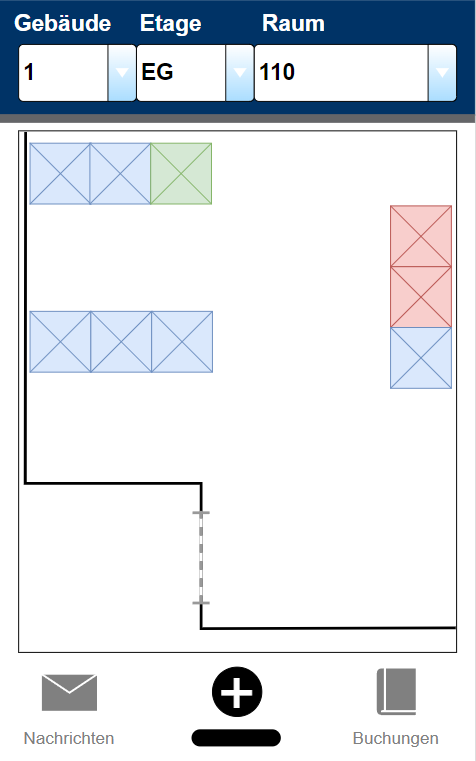
\includegraphics[width=5.5cm]{sketchBooking.png}
  \caption{User Interface: Buchen}
\end{wrapfigure}

Nachfolgend werden die Funktionen und Seiten des mobile first User Interfaces visualisiert und erläutert. 

\subsection{Buchen}

Sobald die Anwendung abgerufen wird, erscheint das Buchen-Fenster.
\paragraph{}Ersichtlich ist das aktuell geöffnete Fenster durch die Funktionsleiste am unteren Ende der Anwendung. 
Dort wird die ausgewählte Funktion, sprich das aktuelle Fenster, durch die dunkel schwarze Färbung und den Balken darunter hervorgehoben.
\paragraph{}Im oberen Teil der Anwendung ist es möglich über Dropdown-Menüs das Gebäude, die Etage und den Raum rauszusuchen, in dem die Buchung gewünscht ist.
Dabei geschieht die Auswahl von rechts startend aus, spricht zuerst das Gebäude, dann die Etage und zuletzt den Raum.
Dies ist wichtig, weil je nach Gebäude andere Etagen bestehen, welche dann wieder nur bestimmte Räume enthalten.

\paragraph{}Wenn im oberen Teil alle Angaben bis zum Raum hin gegeben wurden, erscheint in der Mitte der Anwendung der ausgewählte Raum.
Dieser wird durch ein Rechteck mit dünnen  schwarzen Linien in der Anwendung begrenzt.
In diesem Rahmen soll es möglich sein den Raum zu verschieben und zu vergrößern und zu verkleinern.
Der Raum an sich besteht zum einen aus Wänden, dicke schwarze Striche, und Türen, grau gestrichelte Einsätze in den Wänden. Türen und Wände werden 
lediglich zur Orientierung und besseren Vorstellung des Raumes genutzt. 
\paragraph{}In dem Raum befinden sich schließlich farbige Rechtecke, welche Arbeitsplätze darstellen, welche zum Interagieren benutzt werden. Die farbliche Kennzeichnung beschreibt, wie der Platz an dem heutigen Tag genutzt wird.
Blau zeigt an, dass der Platz frei verfügbar ist für heute, rot zeigt an, dass der Platz mindestens in einem Zeitfenster von heute eine Buchung eines anderen Arbeitskollegen vorliegen hat und grün zeigt an, dass der Arbeitsplatz für heute selbst in mindestens einem Zeitfenster gebucht ist.
\paragraph{}Um weitere und genauere Informationen über die Belegung eines Arbeitsplatzes zu erhalten, wird dieser angeklickt .

\begin{wrapfigure}[21]{l}{5.5cm}
  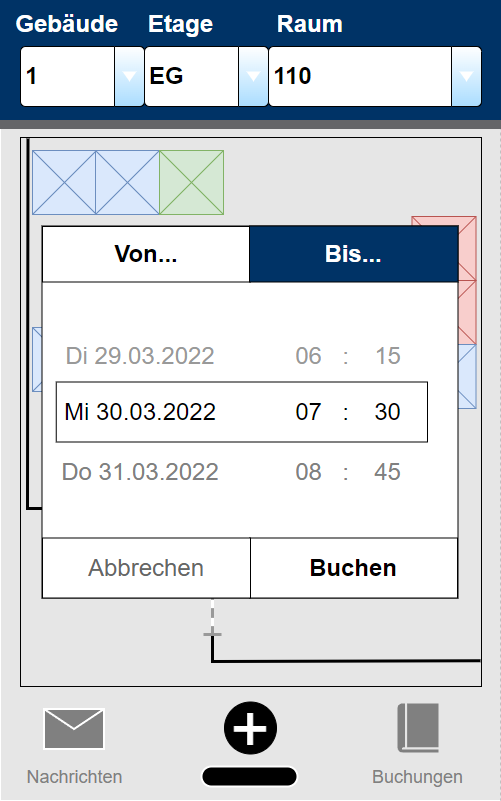
\includegraphics[width=5.5cm]{sketchTime1.png}
  \caption{User Interface: Buchen - Zeitauswahl}
\end{wrapfigure}

\paragraph{}Mit dem Anklicken erscheint ein Pop-Up Fenster, für die Zeiteingabe. 
In der Mitte des Fensters befindet sich die Zeitangabe, die aktuell ausgewählt ist. 
Durch unabhängiges hoch- und runterswipen des Datums, der Stunden und Minuten verändert sich die Zeitangabe.
Die Zeitangaben sind dabei in 15-Minutenschlitze unterteilt.

\paragraph{} Zu Beginn startet das Pop-Up mit der "`Von"' Zeitangabe, welche den Start des Buchungszeitraumes festlegt. 
Im oberen Teil des Pop-Ups wird durch blaue Farbe hervorgehoben, ob es sich um die Eingabe der Startzeit oder der Endzeit handelt.
Mit einem Klick auf "`Von..."' oder "`Bis..."' lassen sich somit auch die Zeiteingaben dafür wechseln. 

\paragraph{}Im unteren Teil des Pop-Ups sind sets die Eingaben verwerfbar durch einen Klick auf "`Abbrechen"'.
Rechts daneben sind die Eingaben zu bestätigen und abzuschicken durch einen Klick auf "`Buchen"'.
Dabei ist der Buchen-Button bei nur einer "`Von"' Angabe noch ausgegraut und nicht anklickbar.
Erst nach der Auswahl der Startzeit und der Endzeit kann der Buchen-Button geklickt werden.

\begin{figure}[!h]
  \centering
  \includegraphics[width=1\textwidth]{sketchTime23.png}
  \caption{User Interface: Buchen - Informationen aus der Zeitauswahl}
  \label{fig:sketch_time_23}
\end{figure}

\paragraph{}Aus der Zeitauswahl folgen noch weitere Informationen dazu ob ein Arbeitsplatz zu einem Zeitpunkt von jemand Anderen gebucht, frei oder selbst gebucht ist. \\
Schwarze Zeitangaben sind frei verfügbar und können ohne Weiteres gebucht werden. \\
Grüne Zeitangaben symbolisieren eigene Buchungen im System. \\
Diese dienen lediglich zur eigenen Information und besitzen keine weiteren Interaktionsmöglichkeiten.\\
Rote Zeitangaben sind von einem Kollegen gebucht, dieser Kollege wird auch in dem Pop-Up Fenster angezeigt.
Anstatt dem Buchen-Button kann der Kollege nun per Nachricht angeschrieben werden, falls der Arbeitsplatz beispielsweise persönlich benötigt wird. 

\subsection{Buchungen/Chronik}

\begin{wrapfigure}[20]{r}{5.5cm}
  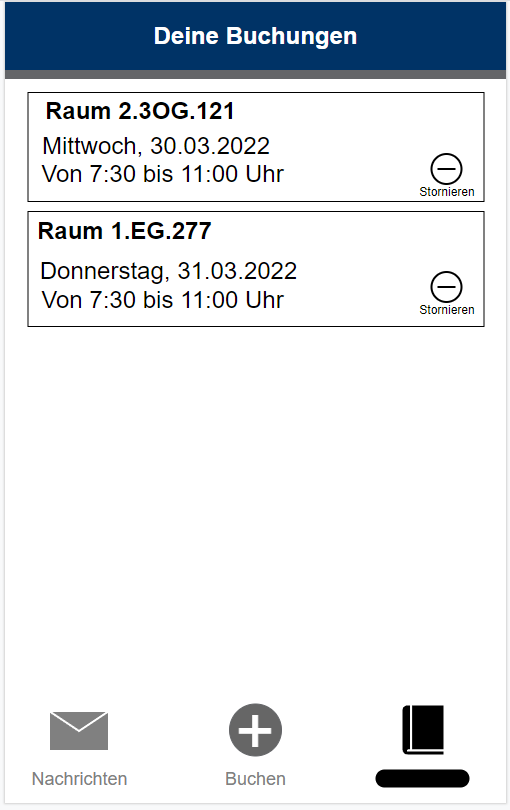
\includegraphics[width=5.5cm]{sketchBuchungen.png}
  \caption{User Interface: Übersicht getätigte Buchungen}
\end{wrapfigure}

Durch einen Klick auf das Buch in der Funktionsleiste unten, geschieht ein Wechsel in die Übersicht aller getätigten Buchungen.
Die Buchungsübersicht wird in Abbildung 9 dargestellt und wird ebenfalls wieder durch die schwarze Färbung des Symbols in der Funktionsleiste und dem Balken darunter hervorgehoben. \\
\paragraph{}In diesem Fenster werden alle Buchungen als Kacheln angezeigt, welche im System getätigt wurden.
Dabei umfasst jede Kachel den Raum, in dem die Buchung gemacht wurde, das Datum und den Zeitraum der gebucht wurde. \\
\paragraph{}In diesem Fenster lässt sich auch jede getätigte Buchung wieder stornieren durch einen Klick auf das Minus-Symbol.

\newpage
\subsection{Nachrichten}

\begin{wrapfigure}[23]{l}{5.5cm}
  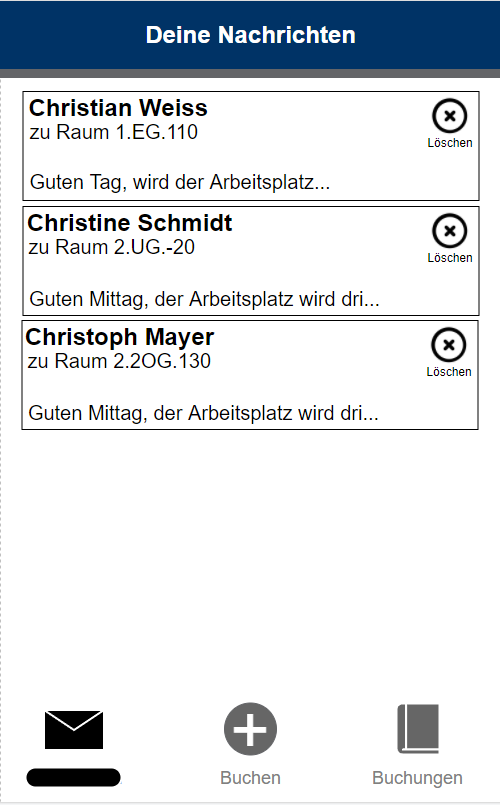
\includegraphics[width=5.5cm]{sketchNachrichten.png}
  \caption{User Interface: Nachrichtenübersicht}
\end{wrapfigure}

Mit einem Klick auf das Briefsymbol, links in der Funktionsleiste, wechselt die Anwendung zur Nachrichtenübersicht.
Dieses Symbol zeigt auch mit einer kleinen hochgestellten Zahl neben dem Icon an, dass ungelesene Nachrichten eingegangen sind.
\paragraph{}Die Nachrichtenübersicht enthält sämtliche Chats, die selbst gestartet wurden oder an einen persönlich gerichtet sind. 
Denn wie zuvor schon erwähnt, besteht die Möglichkeit, Kollegen eine Nachricht zu schreiben, wenn diese einen Arbeitsplatz gebucht haben, der jedoch selbst benötigt wird. 
Dies geschieht über die Zeitraumeingabe, beim Klicken des "`Benachrichtigen"' Buttons, wenn ein Arbeitsplatz, zur gewünschten Zeit, belegt ist.
\paragraph{} Die Nachrichtenübersicht enthält, wie bei der Buchungsübersicht, ebenfalls alle offenen Chats als Kacheln aufgelistet. 
Diesmal enhalten die Kacheln den Namen des anderen Chatteilnehmers, den Raum in dem die betroffene Buchung ist und den Textanfang der neusten Nachricht im Chat.
Chatkacheln mit ungelesenen Nachrichten werden zudem noch hervorgehoben.

\paragraph{} Für mehr Übersichtlichkeit in der Nachrichtenübersicht ist der Chat löschbar.
Dieser sollte aber jediglich gelöscht werden, wenn das Thema des jeweiligen Chats sich erledigt hat.
Dazu lässt sich jeder Chat löschen, mit einem Klick auf das X-Symbol der jeweiligen Kachel.
Dies löscht den Chat nur persönlich und nicht für den anderen Chatteilnehmer, dieser kann den Chat solange einsehen, bis er ihn auch löscht.

\newpage
\begin{wrapfigure}[15]{r}{5.5cm}
  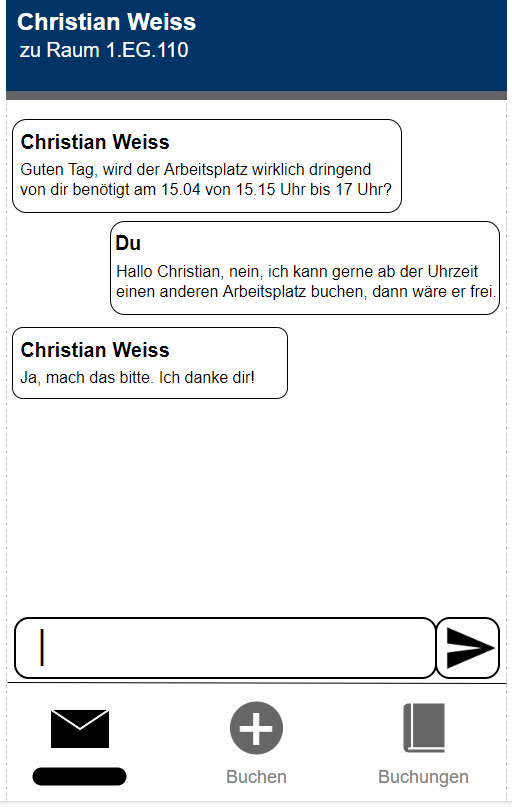
\includegraphics[width=5.5cm]{sketchChat.png}
  \caption{User Interface: Beispielchat}
\end{wrapfigure}

Durch das Anklicken einer Kachel in der Nachrichtenübersicht in Abbildung 10, erscheint der Chat inklusive Chatverlauf.
Der Chat ist in Abbildung 11 dargestellt.

\paragraph{} Im Kopf des Chats sind nochmal die gleichen Informationen, wie in der Übersicht, bisauf den Anfang der neusten Nachricht. 
Direkt darunter ist der Chatverlauf.
Eigene Nachrichten sind hierbei nach rechts verschoben und Nachrichten des Gegenüber nach links.

\paragraph{}Überhalb der Funktionsleiste ist noch die Eingabeleiste, welche durch Anklicken das Verfassen einer Nachricht ermöglicht. 
Die Eingabeleiste öffnet hierbei schließlich die Texteingabe des Gerätes.
Nach fertigem Verfassen der Nachricht kann diese abschickt werden mit dem Symbol rechts neben der Eingabeleiste. 

\vspace{5cm}

\section{Administrator User Interface}

Nachfolgend wird auf das Interface für Administratoren und Geschäftsführer eingegangen. 
Dies wird genutzt um neue Räume im System zu registrieren, zu löschen und zu bearbeiten.
Ebenfalls lassen sich dort Nutzergruppen verwalten, die bestimmen, welcher Mitarbeiten in welchem Raum buchen kann. 

\newpage
\subsection{Raum-Editor}
Die genannten Aufgaben des Administrator User Interfaces lassen sich in dem Editor, in Abbildung 12, vornehmen.

\begin{figure}[!h]
  \centering
  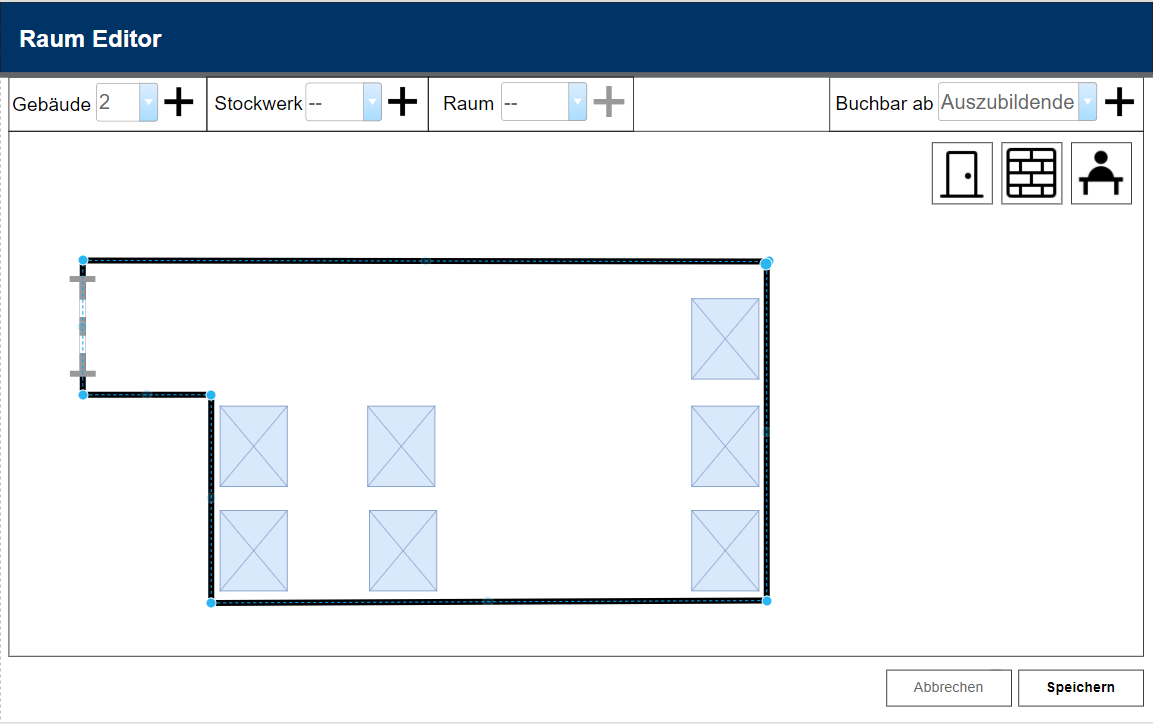
\includegraphics[width=1\textwidth]{sketchEditor.png}
  \caption{User Interface: Raum-Editor}
  \label{fig:sketch_RaumEditor}
\end{figure}

Von oben nach unten durchgehend, werden nachfolgend die Funktionen des Editors erklärt.
\\
Oben links besitzt der Editor Auswahlmöglichkeiten für das Gebäude, die Etage und den Raum.
Ausgewählt wird über Dropdown Menüs, welche von links nach rechts ausgewählt werden müssen, wie in der normalen Raumwahl im Buchen Fenster.
Mit einem Rechtsklick auf Einträge im Dropdown Menü lassen sich Räume löschen.
Über das Plus-Symbol rechts neben dem Dropdown Menü kann ein neuer Eintrag jeweils zum System hinzugefügt werden.
Dabei ist es so, dass immer ein Gebäude hinzugefügt werden kann, da dies nicht von vorherigen Auswahlen abhängt. 
Um eine Etage hinzuzufügen, muss ein Gebäude ausgewählt sein, damit die Etage dem ausgewählten Gebäude zugeordnet werden kann.
Zuletzt kann ein Raum hinzugefügt werden, indem ein Gebäude und eine Etage ausgewählt ist.
\\
Bei sämtlichem Hinzufügen erscheint eine Eingabeleiste für den Namen des Eintrags.
Die Eingabe bestätigt sich schließlich mit Klicken von "`Ok"' und verwerft sich mit dem Klicken des X-Symbols.

\paragraph{} Ist nun einen Raum ausgewählt oder in der Neuerstellung soweit, dass das Layout angepasst werden kann, kann oben rechts die Gruppe auswählen werden, ab welcher der Raum buchbar ist.
Dies geschieht ebenfalls über ein Dropdown Menü und mit dem Plus-Symbol kann eine neue Benutzergruppe hinzugefügt werden. 

\paragraph{}Mit dem Auswählen oder Erstellen eines Raumes, wird dieser auch unterhalb der oberen Leiste angezeigt. 
In dem Rechteck mit den dünnen schwarzen Linien, lässt sich der Raum interaktiv bearbeiten.
\\
Oben rechts in der Bearbeitungsfläche sind die drei Objekte, die sich beliebig oft in den Raum ziehen lassen.
Nämlich Türen, Wände und Arbeitsplätze.
Die Visualisierung von Türen, Wänden und Arbeitsplätzen ist in "`3.1.1 Buchen"' beschrieben
\\
Türen lassen sich auf bestehende Wände draufziehen, skalieren und verschieben.
Wände lassen sich einfach in die Bearbeitungsfläche ziehen und wie Polygonlinienzüge anpassen.
Arbeitsplätze werden in den Raum reingezogen und können dort auch noch verschoben und skaliert werden.
Die Elemente in der Bearbeitungsfläche lassen sich generell anklicken und bearbeiten.
Mit der Entf. Taste lässt sich das angeklickte Element auch löschen.

\paragraph{} Unten rechts sind letztlich die Änderungen an einem Raum komplett verwerfbar durch "`Abbrechen"'
oder eben speicherbar mit "`Speichern"'.
Nach dem Speichern wird der Raum auch direkt ins System eingefügt.

\paragraph{} Unten links ist nun noch ein Button für die Benutzerverwaltung.
Mit einem Klick auf diesen öffnet sich ein Pop-Up, in welchem die Mitarbeiter den Berechtigungsgruppen zugewiesen werden können.

\newpage
\subsection{Benutzerverwaltung}

\begin{wrapfigure}[20]{r}{5.5cm}
  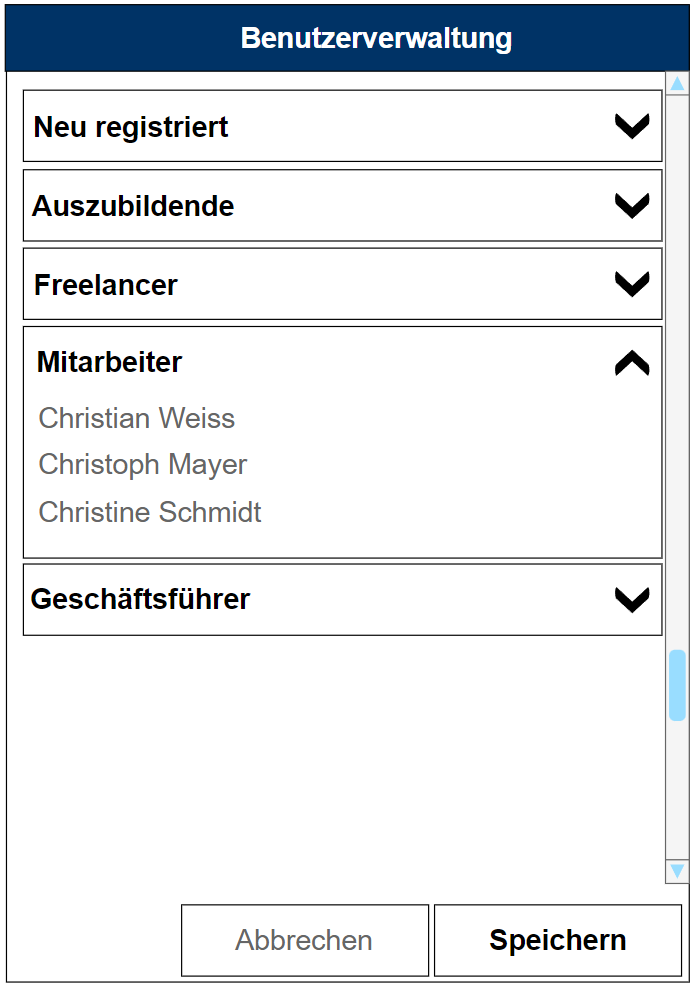
\includegraphics[width=5.5cm]{sketchBenutzerverwaltung.png}
  \caption{User Interface: Benutzerverwaltung Pop-Up}
\end{wrapfigure}

Das Pop-Up für die Gruppenverwaltung und Nutzerzuweiungen in die Gruppen wird in Abbildung 13 beschrieben.
\\
\paragraph{}Hier sind alle Gruppen ersichtlich, die bisher erstellt wurden.
Die Gruppen sind per per Drag and Drop neu sortierbar, damit eine hierarchisch Struktur entsteht.
Dabei ist die niedrigste Hierarchistufe oben und die höchste unten. 
Eine höhere Stufe besitzt dabei jede Zugangsberechtigung der Stufen unterhalb dieser. 
\\
\paragraph{}Die Gruppen können auch aufgeklappt werden, wodurch die jeweiligen Benutzer in dieser Gruppe angezeigt werden.
Diese sind ebenfalls per Drag and Drop in andere Gruppen verschiebbar.
\\
\paragraph{}Nach den getätigeten Änderungen sind diese speicherbar oder verwerfbar. 